% ============================================================================
% SJJI — MICCAI 2026 AMAI workshop submission (Springer LNCS, 8 pages)
% Target: https://sites.google.com/view/amai2026/home  ·  Deadline: June 25, 2026
%
% This file is our drafted CONTENT. Get the official Springer LNCS template + the
% submission rules from paper/README.md (it links the AMAI CFP and the shared Overleaf).
% KEY RULES: 8 pages + up to 2 ref pages · DOUBLE-BLIND (no author names/affiliations,
%   no public-repo link in the PDF) · include the bold "Prospects of Application"
%   paragraph (<= 60 words) at the end of the last section (drafted below).
%   - Sections marked  % >>> TASK: ...  are open pieces — see HANDOFF_SAANVI.md / HANDOFF_ALEX.md.
%   - Our sections (Methods/Results/Discussion/etc.) are drafted — edit for polish only.
% Citations: add entries to refs.bib and cite with \cite{key}.  VERIFY every reference.
% ============================================================================
\documentclass[runningheads]{llncs}
\usepackage{graphicx}
\usepackage{booktabs}
\usepackage{amsmath}
\usepackage[hidelinks]{hyperref}
\graphicspath{{figures/}}

\begin{document}

\title{Site Confounds, Calibration, and the Limits of Self-Supervision in Cross-Dataset Parkinson's EEG Detection}
% DOUBLE-BLIND: keep authors/affiliation anonymized in the SUBMITTED pdf.
% >>> TASK (Edward): real author list + affiliations for the camera-ready only.
\author{Anonymous for review}
\institute{Affiliation withheld for double-blind review}
\maketitle

\begin{abstract}
Electroencephalography (EEG) is a low-cost, non-invasive candidate biomarker for Parkinson's disease (PD), and deep-learning models report high balanced accuracy on a benchmark that pools four public PD datasets. We show that this pooled accuracy is largely a \emph{site artifact}: because the datasets have strongly imbalanced, dataset-specific label distributions, a site-prior null that uses no EEG signal---predicting each dataset's majority class---reaches 0.927 segment-level balanced accuracy, matching or exceeding published models. Evaluating instead with leave-one-dataset-out (LODO), where the test site is unseen, fixed-threshold balanced accuracy collapses toward chance. We demonstrate this collapse is primarily a \emph{calibration failure under domain shift, not an absence of signal}: supervised representations rank PD versus healthy controls on unseen sites at ROC-AUC $0.76\pm0.03$, and a fully deployable decision threshold---selected on the training sites---recovers $0.64\pm0.03$ balanced accuracy. Finally, self-supervised pretraining does not improve cross-site transfer at the scales tested: pretraining on the four datasets or on a large disjoint clinical corpus (TUH) yields cross-site AUC of 0.58 and 0.53 respectively, far below the supervised model, with no advantage in fine-tuning or data-efficiency. We release the evaluation tooling and argue that cross-site PD-EEG should be reported with LODO, threshold-independent metrics, and an explicit site-prior null.
\keywords{EEG \and Parkinson's disease \and cross-site generalization \and dataset confound \and calibration \and self-supervised learning.}
\end{abstract}

% ============================================================================
\section{Introduction}
% >>> TASK (Saanvi or Alex): write the opening hook paragraph here — clinical
%     motivation: PD prevalence, late diagnosis from motor symptoms, EEG as an
%     accessible biomarker, and why a model must work across hospitals to matter.
%     ~4--6 sentences. See HANDOFF_SAANVI.md / HANDOFF_ALEX.md.
\textbf{[HOOK PARAGRAPH — Saanvi/Alex]}

Deep-learning models for EEG-based PD detection are commonly evaluated by pooling several public datasets and performing subject-level cross-validation, reporting balanced accuracies near 80--90\%. This protocol holds out subjects but not \emph{sites}: every dataset appears in both training and test folds. Because EEG recordings are trivially identifiable by site (amplifier, montage, filtering) and because each dataset carries a dataset-specific label distribution, a model can achieve high pooled accuracy by recognizing the dataset rather than the disease. Whether such accuracy reflects pathology---and whether it transfers to a genuinely unseen site---has not been directly tested.

We make three contributions. \textbf{(1)} We introduce a \emph{site-prior null} and show that the pooled-protocol accuracy is confounded: a no-EEG baseline matches published models. \textbf{(2)} Using leave-one-dataset-out, we show the resulting cross-site ``failure'' is mostly a calibration problem; supervised representations transfer (AUC $\approx 0.76$) and a deployable threshold recovers useful balanced accuracy. \textbf{(3)} We report a careful negative result: self-supervised pretraining---including on a large disjoint corpus---does not improve cross-site transfer, across linear-probe, fine-tune, and data-efficiency evaluations.

% ============================================================================
\section{Related Work}
% >>> TASK (Saanvi: Track A — EEG eval/site effects + PD-from-EEG ;
%             Alex:  Track B — SSL for EEG + calibration under shift).
%     Source material + the pre-seeded paper list + the closest 2026 competitors
%     are in docs/related_works.md. Write ~1 short paragraph per theme below.
%     CITE the two starred competitor papers and state how we go further
%     (site-prior null / calibration reframe / SSL-negative). VERIFY every citation.
% STATUS: Track B (SSL + calibration) is drafted below, cites verified in refs.bib.
% Track A (Saanvi) is still to do: add the two subsections below and cite the two
% 2026 competitor papers listed in docs/related_works.md.
\textbf{[RELATED WORK: Track A (Saanvi) still to be written. Track B drafted below.]}

% \subsection{EEG-based Parkinson's detection.}        % Saanvi -- TODO
% \subsection{Evaluation pitfalls and site effects in EEG-DL.}  % Saanvi -- TODO

\subsection{Self-supervised learning for EEG.}
Self-supervised pretraining has produced several EEG ``foundation models'' that learn from large unlabeled corpora and then transfer to downstream tasks. BENDR adapts a wav2vec-style contrastive objective to large EEG collections~\cite{bendr2021}, and BIOT tokenizes heterogeneous biosignals so that datasets with mismatched channels can be trained together~\cite{biot2023}. More recent models such as LaBraM~\cite{labram2024}, EEGPT~\cite{eegpt2024}, and CBraMod~\cite{cbramod2025} scale masked pretraining to thousands of hours and report strong results across many benchmarks, and a recent survey treats self-supervision as the main answer to EEG's shortage of labels~\cite{weng2024sslsurvey}. On clinical EEG, Banville et al.~\cite{banville2021} find that self-supervised features help most when labels are scarce, which is the regime our data-efficiency experiment targets. Our own pretraining follows this line, using VICReg~\cite{vicreg2022} through the SelfEEG library~\cite{selfeeg2024}.

The closest prior work is MCLPD, which applies multi-view contrastive pretraining to cross-dataset Parkinson's EEG and reports that self-supervision improves leave-one-dataset-out transfer~\cite{mclpd2025}. We read that claim with some caution, because several recent evaluations report that EEG foundation models add little over compact supervised baselines~\cite{lee2025lbm}, and that on standardized benchmarks models trained from scratch stay competitive while larger models do not transfer any better~\cite{liu2026eegfm}. The pattern is not specific to EEG. With careful model selection, plain empirical risk minimization matches specialized domain-generalization methods~\cite{gulrajani2021}, and pretraining tends to correct poor extrapolation without removing dataset-specific biases or spurious correlations~\cite{cohenwang2024}. That last point matters here, since self-supervision has also been reported to improve robustness under shift~\cite{hendrycks2019ssl}, which is part of why we expected it to help. None of these studies measure whether self-supervision improves cross-site transfer under a strict leave-one-dataset-out clinical protocol. We run that test and find no benefit at the scale available to us, including when pretraining on a large clinical corpus that shares no recordings with the evaluation data.

\subsection{Calibration under domain shift.}
Modern neural networks are frequently overconfident, and simple post-hoc methods such as temperature scaling~\cite{guo2017calibration} or isotonic regression~\cite{zadrozny2002} usually correct this at low cost. The problem is harder once the test distribution differs from training. Ovadia et al.~\cite{ovadia2019} show that accuracy and calibration both degrade under shift, and that a calibrator fit in-distribution does not carry over to shifted data. Two results are closer to what we need. Yu et al.~\cite{yu2022multidomain} fit temperature scaling across several training domains to obtain a calibrator that holds up under shift, which is essentially our situation with several training hospitals. Wald et al.~\cite{wald2021} connect calibration across domains to out-of-domain generalization and use a robust form of isotonic regression for post-processing. Prevalence shift is a related concern in clinical use: when the positive rate at the deployment site differs from training, the best decision threshold moves and fixed-threshold scores become misleading. Godau et al.~\cite{godau2023} restore reasonable decisions by setting the operating point from the deployment prevalence without using target labels, which is what our prevalence-matched and train-transferred thresholds do. We take the same view for cross-site Parkinson's EEG. The apparent leave-one-site-out failure is mostly a thresholding problem, and a threshold or recalibration fit only on the training sites, never touching the held-out labels, recovers most of the balanced accuracy that is actually achievable.

% ============================================================================
\section{Methods}

\subsection{Datasets.}
We use four public OpenNeuro PD datasets (270 subjects: 140 PD, 130 healthy controls [HC]) and the Temple University Hospital (TUH) EEG corpus as an unlabeled pretraining source. The labeled datasets differ markedly in composition: ds004148 contributes 60 HC and no PD; ds002778 (UC San Diego) 15 PD / 16 HC; ds003490 (UNM 3-Stim) 25 PD / 25 HC; and ds004584 100 PD / 49 HC. After windowing, ds004148 alone accounts for 12{,}369 of 18{,}721 segments (66\%), all HC---a composition central to the confound in Section~\ref{sec:confound}.

\subsection{Preprocessing and channel harmonization.}
Recordings are band-pass filtered (1--45\,Hz), resampled to 250\,Hz, segmented into 16\,s windows with 25\% overlap, and z-scored per channel within each segment (no statistics shared across the train/test boundary). The original benchmark uses the 29 channels common to all four OpenNeuro datasets; however, measuring channel presence directly on TUH shows only 15 of these 29 carry signal (ten extended 10--10 positions are absent; four appear under legacy names T3/T4/T5/T6). We add an old-to-new name remap and adopt the \textbf{19-channel TUH$\cap$OpenNeuro montage} (verified present in TUH), so a TUH-pretrained encoder never learns channel filters on dead inputs. All cross-site experiments use the 19-channel montage.

\subsection{Architecture.}
We use the TransformEEG encoder (depthwise convolutional tokenizer $\rightarrow$ two-layer transformer $\rightarrow$ adaptive pooling), producing a $C\times 4$ feature. A two-layer head is attached for supervised training; a VICReg projector for self-supervised pretraining.

\subsection{Evaluation protocols.}
\textbf{Combined N-LNSO} is the field-standard pooled protocol: all four datasets are merged and 10-fold subject-stratified cross-validation holds out subjects; every dataset appears in every fold. \textbf{Leave-one-dataset-out (LODO)} holds out one entire dataset as the test site and trains on the other three; this removes the site shortcut and is our primary cross-site protocol (the three held-out test sites are the both-class PD datasets). Alongside every pooled number we report a \textbf{site-prior null}: a classifier that predicts the majority class of each test segment's dataset, using no EEG signal, scored on the same metric.

\subsection{Metrics and calibration policies.}
We report subject-level balanced accuracy (segment scores averaged per subject before thresholding) and \textbf{ROC-AUC}, which is threshold-independent. Because a fixed 0.5 threshold mis-calibrates on an unseen site, we evaluate several threshold policies: \emph{fixed-0.5}; \emph{train-transferred} (threshold maximizing balanced accuracy on the training sites, applied unchanged---fully deployable); \emph{prevalence-matched} (predicted positive rate set to the held-out site's PD prevalence); and \emph{oracle} (the ceiling implied by the AUC). Variability is mean\,$\pm$\,std across three seeds.

\subsection{Self-supervised pretraining.}
We pretrain with VICReg and evaluate three ways: a \textbf{linear probe} (encoder frozen), \textbf{fine-tuning} (encoder initialized from the SSL checkpoint, trained end-to-end), and a \textbf{data-efficiency} sweep (fine-tuning on 10/25/100\% of training subjects). We pretrain on two sources: the four OpenNeuro datasets (labels ignored) and a disjoint TUH subset (298 recordings, 19{,}883 segments) sharing no recordings with evaluation data. Supervised/fine-tuning runs use Adam ($\beta_1{=}0.75$), lr $2.5\times10^{-4}$, 50 epochs.

% ============================================================================
\section{Results}

\subsection{The pooled-protocol accuracy is a site artifact.}\label{sec:confound}
On combined N-LNSO, the supervised model reaches 0.89 median segment-level balanced accuracy and the SSL probe 0.90--0.92. However, the \textbf{site-prior null reaches 0.927} (segment) and 0.654 (subject) using no EEG signal (Fig.~\ref{fig:confound}). Because ds004148 is entirely HC and dominates the segment pool while each PD dataset is PD-majority, predicting the dataset's majority class alone matches or exceeds the trained models. The pooled metric therefore cannot distinguish ``detects Parkinson's'' from ``detects the dataset.''

\subsection{Honest cross-site evaluation: calibration, not absent signal.}
Under LODO, fixed-0.5 subject-level balanced accuracy is $0.585\pm0.014$---near chance, predicting PD for almost all subjects on an unseen site. Yet the threshold-independent \textbf{ROC-AUC is $0.763\pm0.034$} (Fig.~\ref{fig:ssl}): the model ranks PD above HC well above chance on sites it never saw. The collapse is a calibration artifact. A threshold chosen on the training sites and transferred (fully deployable) recovers $0.643\pm0.034$; prevalence-matching reaches $0.686\pm0.041$; the oracle ceiling is 0.732 (Fig.~\ref{fig:calib}). Cross-site PD detection is thus real but modest, and bottlenecked by calibration rather than representation. Smarter post-hoc recalibration does not help: temperature scaling cannot move the fixed-0.5 operating point (balanced accuracy stays $0.585$), and Platt and isotonic regression fit on independent sites reach only $0.591$ and $0.629$---none beats the $0.643$ train-transferred threshold~\cite{guo2017calibration,zadrozny2002}. With the AUC fixed, the operating point is the only lever, and a threshold transferred from the training sites already captures most of the recoverable accuracy.

\subsection{Self-supervised pretraining does not improve cross-site transfer.}
SSL fails to help across every evaluation (Fig.~\ref{fig:ssl},~\ref{fig:de}). \emph{Linear probe:} cross-site AUC is $0.581\pm0.002$ (OpenNeuro) and $0.526\pm0.003$ (disjoint TUH), versus 0.763 supervised; the disjoint, larger-corpus encoder is the weakest, consistent with a domain mismatch between clinical TUH EEG and resting-state PD recordings. \emph{Fine-tuning:} initializing from the TUH encoder matches from-scratch at full labels (0.73 vs 0.76). \emph{Data-efficiency:} across 10/25/100\% label budgets and three seeds, SSL-TUH tracks from-scratch at every point (Fig.~\ref{fig:de}); SSL does not lower the label requirement. \emph{Augmentation:} no cross-site lift (0.763 vs 0.764). The negative is stable across seeds (std $\approx 0.002$).

\begin{figure}[t]
\centering
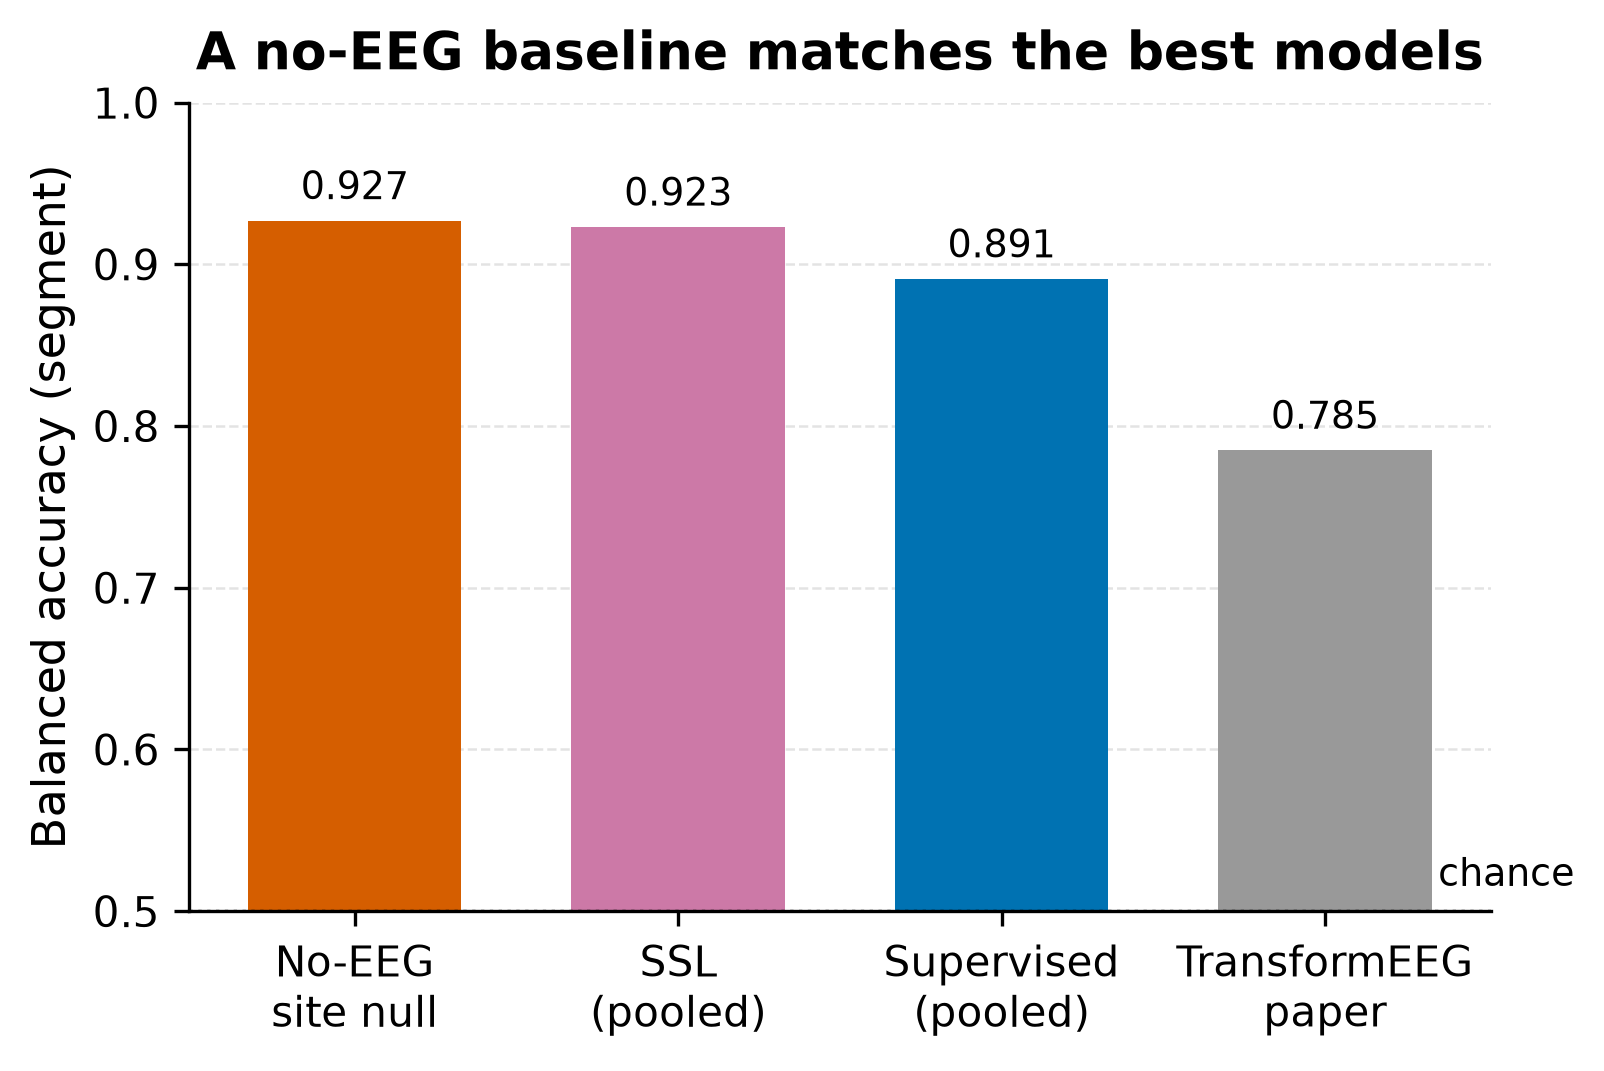
\includegraphics[width=0.49\textwidth]{fig1_confound.png}
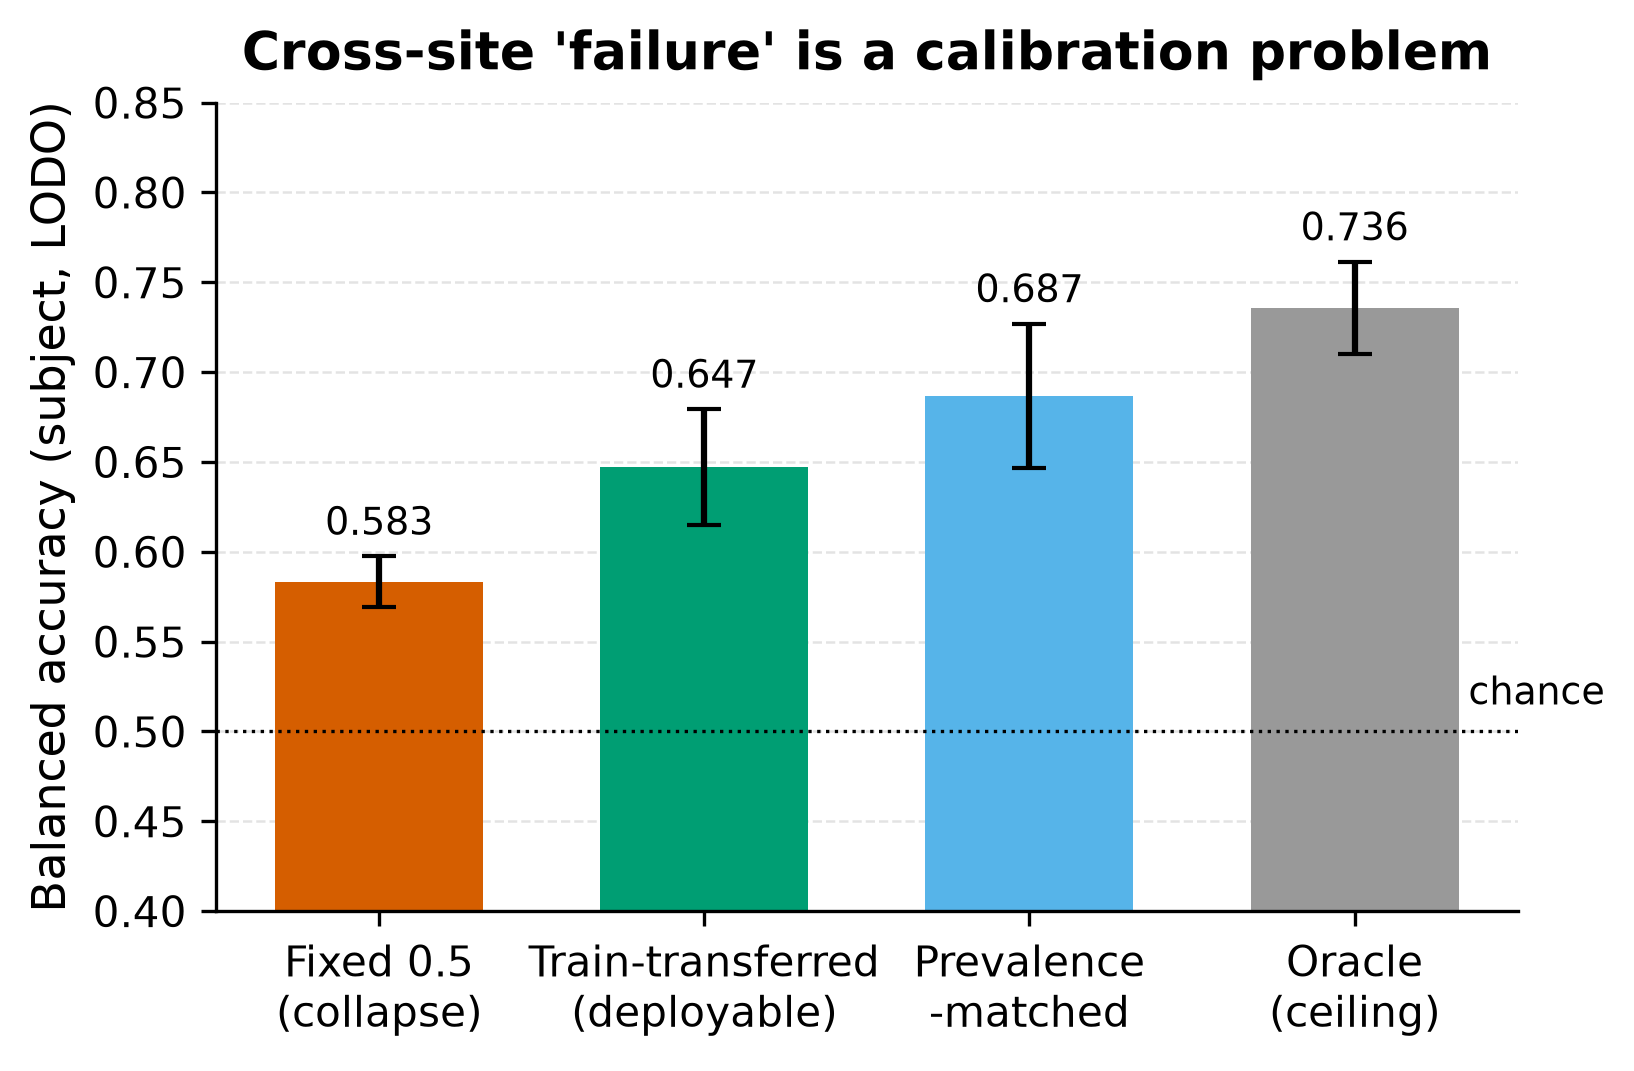
\includegraphics[width=0.49\textwidth]{fig2_calibration.png}
\caption{\textbf{Left (Fig.~1):} a no-EEG site-prior null matches the best models on the pooled protocol. \textbf{Right (Fig.~2):} under LODO, a deployable threshold recovers balanced accuracy the fixed-0.5 collapse hides.}
\label{fig:confound}
\label{fig:calib}
\end{figure}

\begin{figure}[t]
\centering
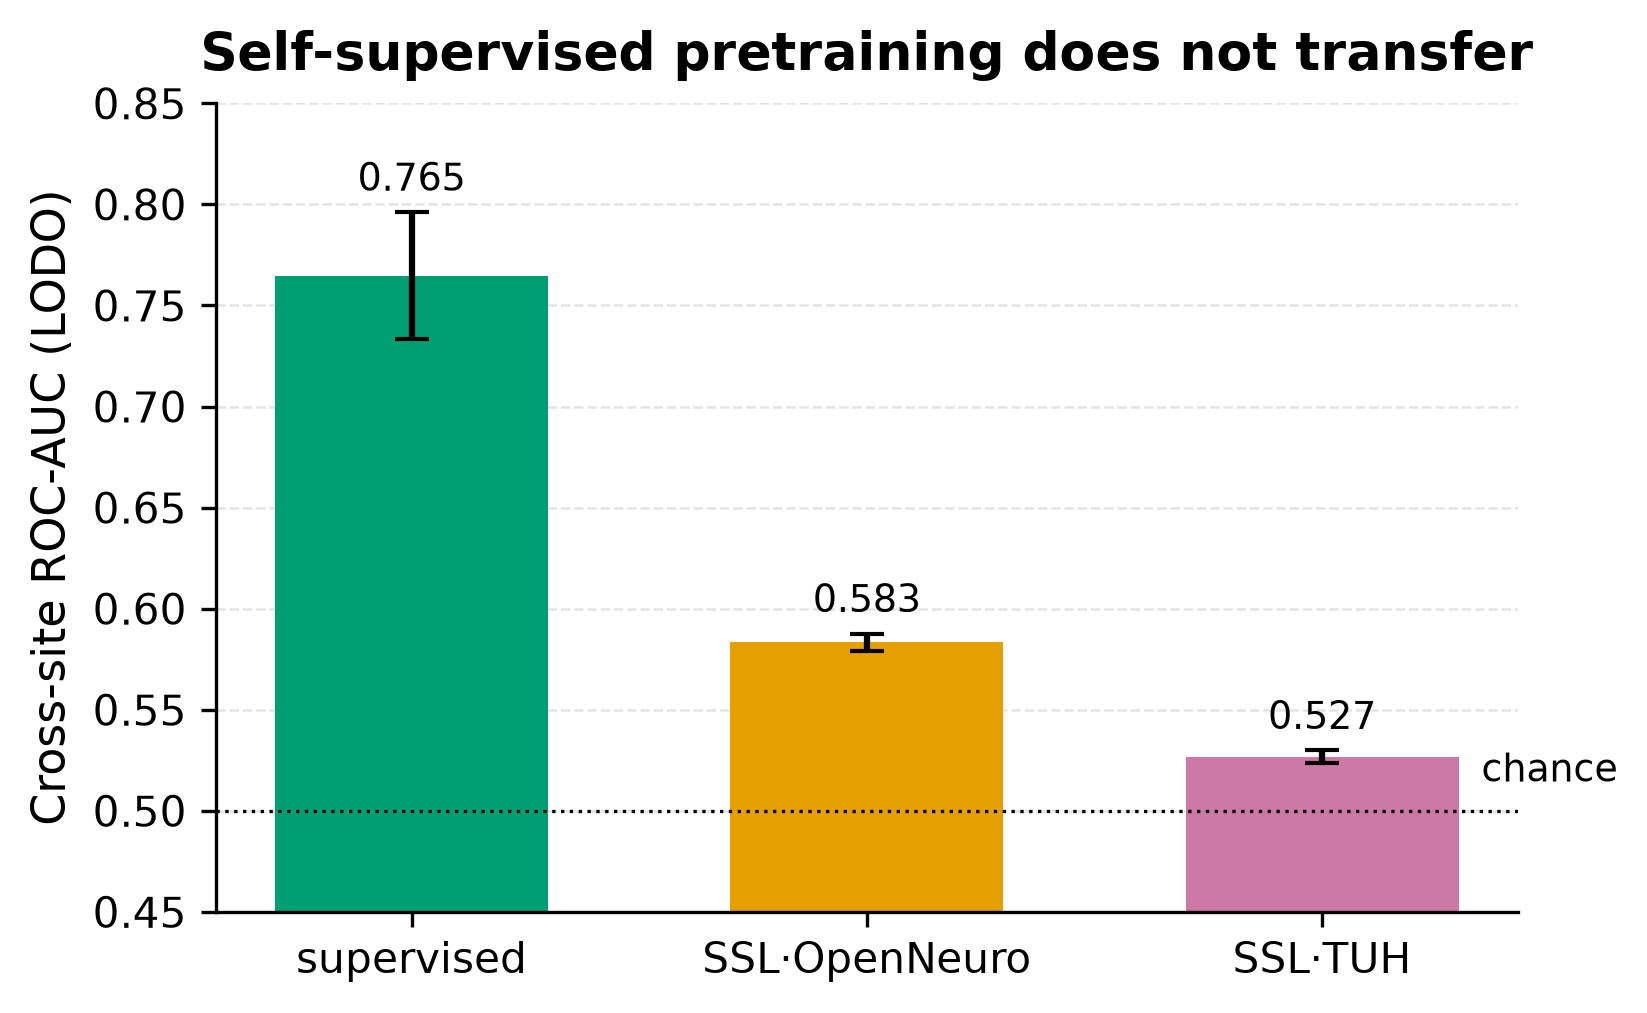
\includegraphics[width=0.49\textwidth]{fig3_ssl_auc.png}
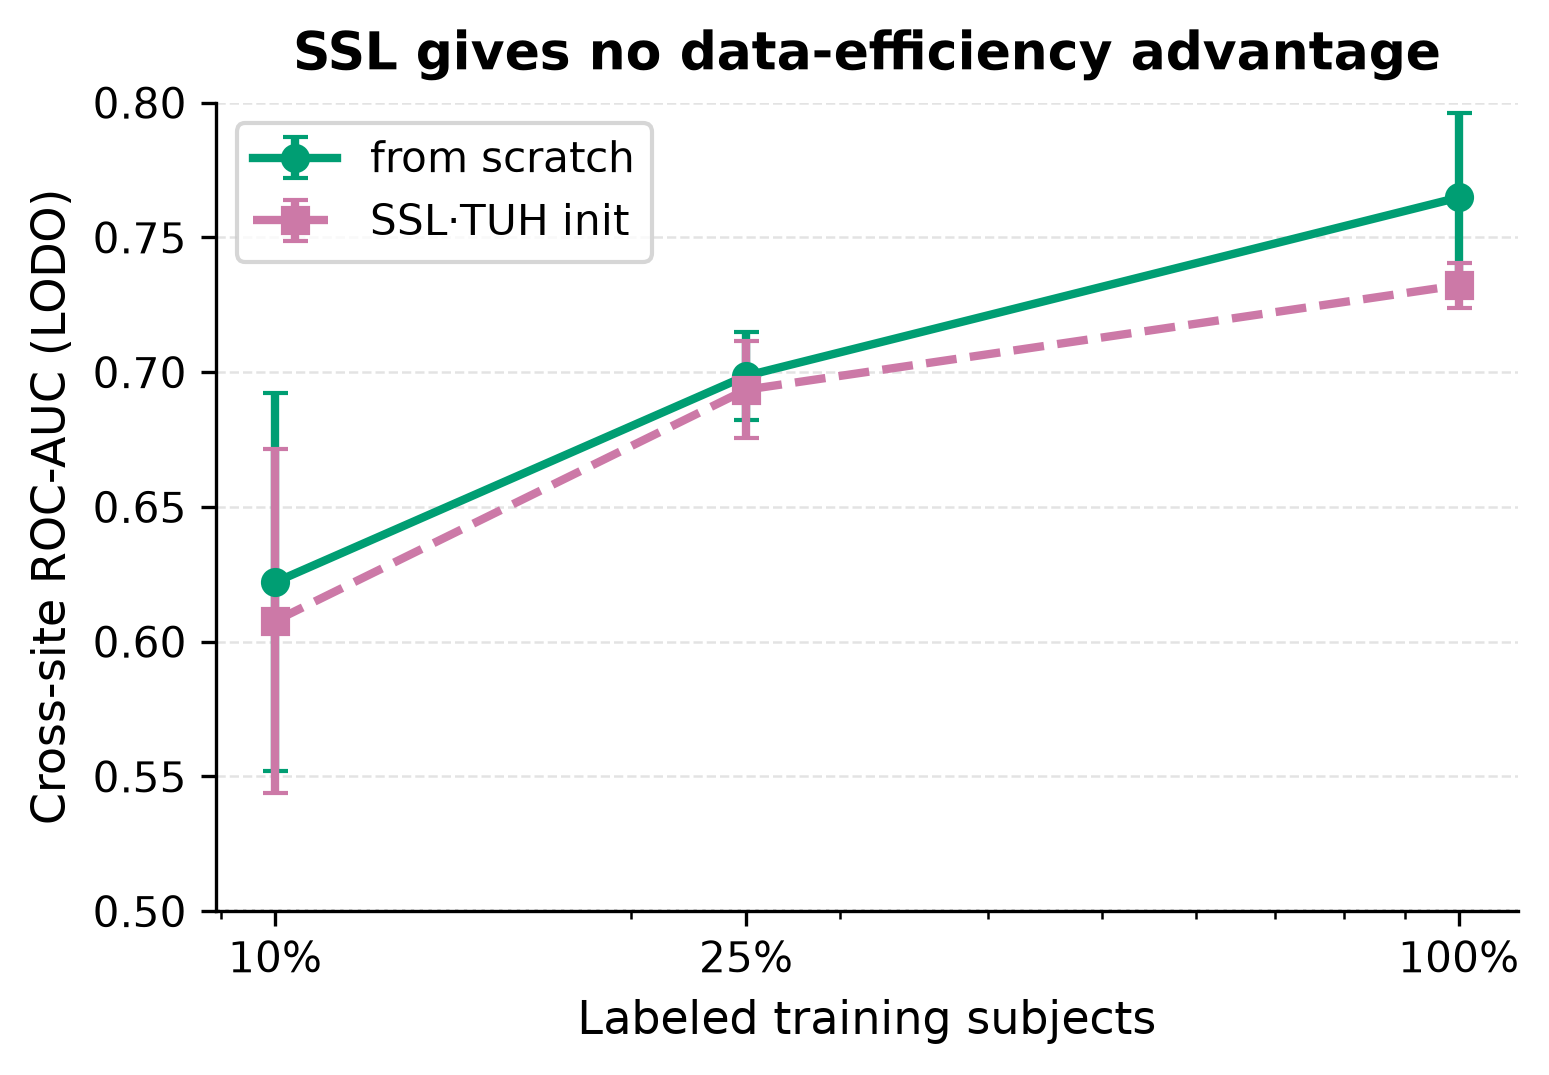
\includegraphics[width=0.49\textwidth]{fig4_data_efficiency.png}
\caption{\textbf{Left (Fig.~3):} cross-site ROC-AUC by method---supervised transfers, SSL does not. \textbf{Right (Fig.~4):} SSL fine-tuning gives no data-efficiency advantage at any label budget.}
\label{fig:ssl}
\label{fig:de}
\end{figure}

% ============================================================================
\section{Discussion}
Our results reframe cross-dataset PD-EEG. First, the widely reported pooled accuracy is substantially a measurement artifact; the appropriate baseline is the site-prior null, and evaluation should hold out whole sites. Second, the apparent cross-site failure of supervised models is largely a \emph{calibration} problem---practically important and partly solvable: a threshold transferred from training sites recovers most of the achievable balanced accuracy, and the residual gap to the oracle motivates site-aware calibration rather than better features. Third, self-supervised pretraining does not deliver a cross-site advantage here, even from a large disjoint corpus and in the fine-tuning and low-label regimes where it is expected to shine; the likely cause is domain mismatch (clinical vs resting-state EEG), suggesting that \emph{what} one pretrains on matters more than scale.

\section{Conclusion}
Cross-dataset PD-EEG accuracy, as conventionally reported, is largely a site artifact. Measured honestly with leave-one-dataset-out, threshold-independent metrics, and an explicit site-prior null, supervised detection transfers across sites at a real but modest, calibration-bound level, and self-supervised pretraining does not improve it at the scales tested.

\noindent\textbf{Prospects of Application.} As a screening aid, EEG-based Parkinson's detection must work at clinics unseen during training. Our results show this is feasible at modest, calibration-dependent accuracy: a model trained on existing datasets transfers (AUC $\approx 0.76$) and, with a site-aware decision threshold, reaches deployable balanced accuracy $\approx 0.64$, whereas conventionally reported pooled accuracies overstate clinical readiness.

\subsubsection*{Limitations.}
Four datasets and three held-out sites; a single architecture; small subject counts per held-out site (31/50/149); SSL pretraining bounded by single-GPU scale (the disjoint TUH subset is $\sim$20k segments). Cross-site and data-efficiency results use three seeds.

% ============================================================================
\bibliographystyle{splncs04}
\bibliography{refs}
% >>> TASK (Saanvi/Alex): build refs.bib in Zotero as you read. Cite with \cite{}.
\end{document}
